%%%%%%%%%%%%%%%%%%%%%%%%%%%%%%%%%%%%%%%%%%%%%%%
% Template baseado no exemplo da classe utftex
% Prof. César M. V. Benítez, Daniel Rossato
% DAELN, UTFPR-Curitiba (2020)
%%%%%%%%%%%%%%%%%%%%%%%%%%%%%%%%%%%%%%%%%%%%%%%


\documentclass[openright]{normas-utf-tex} %openright = o capitulo comeca sempre em paginas impares
%\documentclass[oneside]{normas-utf-tex} %oneside = para numero de paginas menor que 100 (apenas frente da folha) 

% force A4 paper format
\special{papersize=210mm,297mm}

\usepackage[alf,abnt-emphasize=bf,bibjustif,recuo=0cm, abnt-etal-cite=2, abnt-etal-list=99]{abntcite} %configuracao correta das referencias bibliograficas.

\usepackage[portuguese, ruled, linesnumbered]{algorithm2e}%pacotedealgoritmoemportugues

\usepackage[table]{xcolor}
\usepackage[brazil]{babel} % pacote portugues brasileiro
\usepackage[utf8]{inputenc} % pacote para acentuacao direta
\usepackage{amsmath,amsfonts,amssymb} % pacote matematico
\usepackage{graphicx} % pacote grafico
\usepackage{times} % fonte times
\usepackage[final]{pdfpages} % adicao da ata
\usepackage[version=3]{mhchem}%adição de pacote para quimica
% \usepackage{longtable}% redimensionar automaticamente tabelas
\usepackage{subfig}
\usepackage{relsize}
\usepackage[paper=portrait,pagesize]{typearea}
\usepackage{pdflscape}
\usepackage{url}


%\usepackage{hyperref}% link das res
\newcommand\tab[1][1cm]{\hspace*{#1}}

%Podem utilizar GEOMETRY{...} para realizar pequenos ajustes das margens. Onde, left=esquerda, right=direita, top=superior, bottom=inferior. P.ex.:
%\geometry{left=3.0cm,right=1.5cm,top=4cm,bottom=1cm} 
\usepackage{amsthm}
\newtheorem{mydef}{Definicão}

%\usepackage{balance} 



% ---------- Preambulo ----------
\instituicao{ UNIVERSIDADE TECNOLÓGICA FEDERAL DO PARANÁ (UTFPR)} % nome da instituicao
\programa{Curso de Engenharia Eletrônica} % nome do programa
\area{Engenharia Eletrônica} 
\documento{Oficina de Integração -- Relatório Final} % Oficina de Integração
\nivel{Graduação em Engenharia Eletrônica} 
\titulacao{Graduação em Engenharia Eletrônica} 

\titulo{Título em Português} % titulo do trabalho em portugues
\title{\MakeUppercase{Título em Inglês}} % titulo do trabalho em ingles

\autor{Aluno 1 \protect \\ Aluno 2 \protect Aluno 3} % autor do trabalho
%\cita{aluno1} % sobrenome (maiusculas), nome do autor do trabalho


\palavraschave{palavra chave}  % palavras-chave do trabalho
\keywords{keywords} % palavras-chave do trabalho em ingles

\comentario{Relatório Final da disciplina Oficina de Integração, do curso de Engenharia Eletrônica,  apresentado aos professores que ministram a mesma na Universidade Tecnologica Federal do  Paraná como requisito parcial para obtenção da aprovação na disciplina.} 

\orientador{Prof. M.Sc. Daniel Rossato \protect \\ 
Prof. M.Sc. Gabriel Kovalhuk} % nome do orientador do trabalho



\local{Curitiba} % cidade
\data{\the\year} % ano automatico

% desativa hifenizacao mantendo o texto justificado.
% thanks to Emilio C. G. Wille
\tolerance=1
\emergencystretch=\maxdimen
\hyphenpenalty=10000
\hbadness=10000
\sloppy

%---------- Inicio do Documento ----------
\begin{document}

\capa % geracao automatica da capa
\folhaderosto % geracao automatica da folha de rosto


% % dedicatoria (opcional)
\begin{dedicatoria}
% Texto da dedicat\'oria.
Este trabalho é dedicado a \dots 

\end{dedicatoria}

% % agradecimentos (opcional)
\begin{agradecimentos}
% Texto dos agradecimentos.


 \end{agradecimentos}

% % epigrafe (opcional)
% \begin{epigrafe}
% Texto da ep\'igrafe.
% \end{epigrafe}

%resumo
\begin{resumo}

\end{resumo}

%abstract
\begin{abstract}

\end{abstract}

% listas (opcionais, mas recomenda-se a partir de 5 elementos)
\listadefiguras % geracao automatica da lista de figuras
\listadetabelas % geracao automatica da lista de tabelas
%\listadequadros % adivinhe :)
\listadesiglas % geracao automatica da lista de siglas
\listadesimbolos % geracao automatica da lista de simbolos

% sumario
\sumario % geracao automatica do sumario


%---------- Inicio do Texto ----------
% recomenda-se a escrita de cada capitulo em um arquivo texto separado (exemplo: intro.tex, fund.tex, exper.tex, concl.tex, etc.) e a posterior inclusao dos mesmos no mestre do documento utilizando o comando \input{}, da seguinte forma:
%\input{intro.tex}
%\input{fund.tex}
%\input{exper.tex}
%\input{concl.tex}

% Colocar aqui o numero da página inicial!!! (Obs.: conta a partir da folha de rosto)
\setcounter{page}{12}



\chapter{Introdução}

\section{Motivação} %qual o problema?


\section{Objetivos}




\subsection{Objetivo geral} 




\subsection{Objetivos específicos} 
\label{sec:objespecif}

   %Introducao
\chapter{Fundamentação teórica}

Nesta Seção serão apresentadas as diferentes tecnologias disponíveis para resolver cada parte do projeto, seguidas de uma tabela comparativa das principais características, e a escolha justificada. Todas as figuras e tabelas devem ser referenciadas no texto antes de aparecer no documento. A Seção \ref{sec:exemplo} mostra um exemplo resumido do que deve ser feito para cada sensor, módulo, material, etc.

\section{Exemplo de análise de tecnologia - Comunicação sem Fio}
\label{sec:exemplo}
Como mostrado na Seção \ref{sec:objespecif}, o projeto proposto necessita de um módulo de comunicação sem fio para interagir com o aplicativo no celular do usuário. Foram analisadas as tecnologias Wi-Fi e Bluetooth, visto que estas estão presentes em praticamente todos os \textit{smartphones} modernos.

\subsection{Wi-Fi}
\label{sec:wifi}

A tecnologia Wi-Fi é tecnologia de rede sem fio criada em 1998 pela Wi-Fi Alliance, baseada no padrão IEEE 802.11. Ela é hoje a tecnologia mais comum para conexão sem fio de dispositivos à internet em dispositivos pessoais \cite{WiFi2020}. Um dos módulos mais comuns para aplicações de \sigla{IoT}{Internet of Things} (Internet das Coisas) é o ESP8266 \cite{datasheet8266}, que tem baixo custo e fácil disponibilidade de compra. Este módulo é mostrado na Figura \ref{fig:esp8266}.

\begin{figure}[!htb]
	\centering
	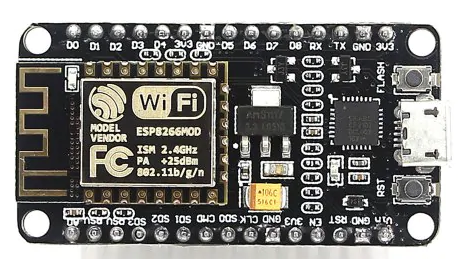
\includegraphics[width=0.4\textwidth]{./esp8266.png} 
	\caption{Foto do módulo Wi-Fi ESP8266.}
	\label{fig:esp8266}
\end{figure}

\subsection{Bluetooth}
\label{sec:bt}
A tecnologia Bluetooth foi criada em 1989, com o objetivo de substituir o protocolo RS-232 na comunicação de curta distância entre objetos fixos (citar referência). O módulo mais comum para IoT é o HC-05, mostrado na Figura \ref{fig:hc05}.

\begin{figure}[!htb]
	\centering
	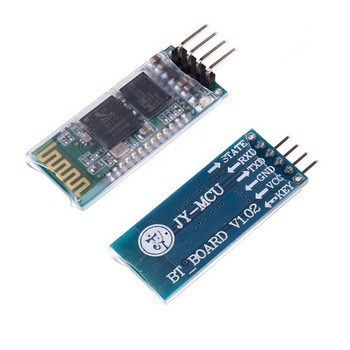
\includegraphics[width=0.4\textwidth]{./hc05.jpg} 
	\caption{Foto do módulo Bluetooth HC-05.}
	\label{fig:hc05}
\end{figure}

\subsection{Comparativo entre tecnologias de comunicação sem fio}
Na Tabela \ref{tab:semfio} são comparadas as principais características dos módulos ESP8266 e HC-05. Esta tabela foi criada com o auxílio do site \url{www.tablesgenerator.com}.

\begin{table}[!htb]
\centering
\begin{tabular}{l|l|l}
    ~       & ESP8266   & HC-05      \\
    \hline
    Alcance & 50m       & 10m        \\
    \hline
    Consumo & 170mA     & 40mA       \\
    \hline
    Preço   & R\$ 22,90 & R\$ 25,90  \\
    \hline
\end{tabular}
\caption{Comparativo entre módulos ESP8266 e HC-05}
\label{tab:semfio}
\end{table}

O módulo ESP8266 tem maior alcance e menor custo que o HC-05, como pode ser visto na Tabela \ref{tab:semfio}. Porém, como o projeto proposto será alimentado por bateria, é essencial diminuir o consumo de corrente do sistema. Por isso, foi escolhido o módulo HC-05. Além disso, o desenvolvimento de aplicações com comunicação Bluetooth já é dominado pela equipe, reduzindo a dificuldade da implementação.



   %Fundamentacao teorica
\chapter{Metodologia}

\section{Visão geral}


* Obs.: nao esqueça de apresentar o diagrama de blocos do sistema. 


\section{Projeto mecânico}


\section{Projeto de \textit{hardware}}


* Obs.: nao esqueça de apresentar o diagrama de blocos do hardware. 


\section{Projeto de \textit{software}}



* Obs.: nao esqueça de apresentar os diagramas de estados (statecharts) do 
software.


\section{Integração}









   %Metodologia
\chapter{Experimentos e resultados}

% testes, integração, etc.   %Experimentos e resultados
\chapter{Cronograma e custos do projeto}

\section{Cronograma}

* Apresentar o cronograma proposto e o final (lista e Diagrama de Gantt). \\


\section{Custos}

* Apresentar o custo do projeto (tabela)   %Cronograma e custos do projeto
\chapter{Conclusões}


\section{Conclusões}



\section{Trabalhos futuros}


%ex.: melhorias,  entre outros.   %Conclusoes e trabalhos futuros






%---------- Referencias ----------
\clearpage % this is need for add +1 to pageref of bibstart used in 'ficha catalografica'.
\label{bibstart}
\bibliography{reflatex} % geracao automatica das referencias a partir do arquivo reflatex.bib
\label{bibend}

% %---------- Apendices (opcionais) ----------
% \apendice
% \chapter{Nome do Ap\^endice}

% Use o comando {\ttfamily \textbackslash apendice} e depois comandos {\ttfamily \textbackslash chapter\{\}}
% para gerar t\'itulos de ap\^en-dices.


% % ---------- Anexos (opcionais) ----------
% \anexo
% \chapter{Nome do Anexo}

% Use o comando {\ttfamily \textbackslash anexo} e depois comandos {\ttfamily \textbackslash chapter\{\}}
% para gerar t\'itulos de anexos.


% --------- Ordenacao Afabetica da Lista de siglas --------
%\textbf{* Observações:} a ordenacao alfabetica da lista de siglas ainda nao eh realizada de forma automatica, porem
% eh possivel se de realizar isto manualmente. Duas formas:
%
% ** Primeira forma)
%    A ordenacao eh feita com o auxilio do comando 'sort', disponivel em qualquer
% sistema Linux e UNIX, e tambem em sistemas Windows se instalado o coreutils (http://gnuwin32.sourceforge.net/packages/coreutils.htm)
% comandos para compilar e ordenar, supondo que seu arquivo se chame 'dissertacao.tex':
%
%      $ latex dissertacao
%      $ bibtex dissertacao && latex dissertacao
%      $ latex dissertacao
%      $ sort dissertacao.lsg > dissertacao.lsg.tmp
%      $ mv dissertacao.lsg.tmp dissertacao.lsg
%      $ latex dissertacao
%      $ dvipdf dissertacao.dvi
%
%
% ** Segunda forma)
%\textbf{Sugest\~ao:} crie outro arquivo .tex para siglas e utilize o comando \sigla{sigla}{descri\c{c}\~ao}.
%Para incluir este arquivo no final do arquivo, utilize o comando \input{arquivo.tex}.
%Assim, Todas as siglas serao geradas na ultima pagina. Entao, devera excluir a ultima pagina da versao final do arquivo
% PDF do seu documento.


%-------- Citacoes ---------
% - Utilize o comando \citeonline{...} para citacoes com o seguinte formato: Autor et al. (2011).
% Este tipo de formato eh utilizado no comeco do paragrafo. P.ex.: \citeonline{autor2011}

% - Utilize o comando \cite{...} para citacoeses no meio ou final do paragrafo. P.ex.: \cite{autor2011}



%-------- Titulos com nomes cientificos (titulo, capitulos e secoes) ----------
% Regra para escrita de nomes cientificos:
% Os nomes devem ser escritos em italico, 
%a primeira letra do primeiro nome deve ser em maiusculo e o restante em minusculo (inclusive a primeira letra do segundo nome).
% VEJA os exemplos abaixo.
% 
% 1) voce nao quer que a secao fique com uppercase (caixa alta) automaticamente:
%\section[nouppercase]{\MakeUppercase{Estudo dos efeitos da radiacao ultravioleta C e TFD em celulas de} {\textit{Saccharomyces boulardii}}
%
% 2) por padrao os cases (maiusculas/minuscula) sao ajustados automaticamente, voce nao precisa usar makeuppercase e afins.
% \section{Introducao} % a introducao sera posta no texto como INTRODUCAO, automaticamente, como a norma indica.

%\balance
\end{document}
